%%%%%%%%%%%%%%%%%%%%%%%%%%%%%%%%%%%%%%%%%%%%%%%%%%%%%%%%%%%%%%%%%%%%%%%
% CACIC 2026 -- formato LLNCS (llncs.cls).
% Reglas de la convocatoria: A4, maximo 10 paginas, sin encabezado ni pie.
% Primera version EN ESPANOL para revision del equipo.
%%%%%%%%%%%%%%%%%%%%%%%%%%%%%%%%%%%%%%%%%%%%%%%%%%%%%%%%%%%%%%%%%%%%%%%
\documentclass{llncs}
\pagestyle{empty}

\usepackage[utf8]{inputenc}
\usepackage[T1]{fontenc}
\usepackage{lmodern}
\usepackage{cmap}
\input{glyphtounicode}
\pdfgentounicode=1
\usepackage[spanish,es-tabla]{babel}
\usepackage{graphicx}
\usepackage{booktabs}
\usepackage{amsmath}
\usepackage{amssymb}
\usepackage{url}
\usepackage{xcolor}
\usepackage{multirow}
\usepackage{etoolbox}
\AtBeginEnvironment{thebibliography}{\footnotesize\setlength{\itemsep}{1pt}}
\usepackage{tikz}
\usetikzlibrary{arrows.meta,positioning}
\usepackage{pgfplots}
\pgfplotsset{compat=1.18}
\usepackage{float}

% Marcador de valor pendiente de medicion. Todo numero que todavia no se midio va
% con esta macro: se ve en rojo y es imposible que se filtre a la version final
% disfrazado de resultado.
\newcommand{\pend}[1][]{\textcolor{red}{\textbf{[pendiente#1]}}}
\newcommand{\nota}[1]{\textcolor{blue}{\textit{[#1]}}}

\begin{document}

% ============================== TITULO ==============================
% Titulo tentativo. Alternativas para discutir:
%   - Usar lo que ya se sabe: metadatos estructurados y estado de dialogo
%     en la recuperacion de normativa universitaria
%   - Quien fijo el valor importa: procedencia del estado de dialogo en un
%     asistente de consulta normativa
\title{Un RAG portable sobre SUDOCU: consulta conversacional de normativa
universitaria mediante estados de di\'alogo con procedencia}
\titlerunning{Un RAG portable sobre SUDOCU}

\author{Juan Manuel Fern\'andez\inst{1} \and
        Francisco Tamasi\inst{1} \and
        Sebasti\'an Marchetti\inst{1} \and
        Mario Oloriz\inst{1} \and
        Marcelo Errecalde\inst{2}}
\authorrunning{J. M. Fern\'andez et al.}
\institute{LICDIA, Universidad Nacional de Luj\'an, Luj\'an, Argentina \and
LIDIC, Universidad Nacional de San Luis, San Luis, Argentina\\
\email{\{jmfernandez,ftamasi,smarchetti,moloriz\}@unlu.edu.ar, merreca@unsl.edu.ar}}

\maketitle
\thispagestyle{empty}

\begin{abstract}
La normativa de las universidades nacionales argentinas es p\'ublica, pero los
portales que la publican solo admiten b\'usqueda por atributos del acto:
localizar qu\'e norma regula una situaci\'on exige conocer de antemano el acto
que la contiene. Se presenta un sistema de generaci\'on aumentada por
recuperaci\'on (RAG) sobre el m\'odulo de publicaci\'on documental de SUDOCU,
desplegado sobre los 21.344 actos administrativos de la Universidad Nacional de
Luj\'an, segmentados por unidad normativa en 151.696 fragmentos. La
recuperaci\'on combina \emph{embeddings} multiling\"ues con un \'indice l\'exico
que preserva los identificadores normativos, fusionados por posici\'on. Sobre
esa base, el sistema mantiene un estado de di\'alogo con dos \emph{slots} ---la
entidad en discusi\'on y los actos mencionados--- cuyo peso en la recuperaci\'on
lo determina la \emph{procedencia} de cada valor: lo que el sistema infiere
pondera d\'ebilmente; lo que el usuario fija, visible y editable en la interfaz,
prevalece y no se sobrescribe. En la evaluaci\'on, el anclaje resuelve por
completo las consultas por identificador (R@5 de 1{,}00), el procesamiento
conversacional lleva la repregunta el\'iptica de 0{,}12 a 0{,}93 y el 97{,}0\%
de los actos citados tiene correspondencia verificada con lo recuperado.
La portabilidad se verific\'o construyendo una segunda instancia sobre el portal
de la Universidad Nacional de San Luis, con el mismo c\'odigo y solo
configuraci\'on.

\keywords{RAG, SUDOCU, Estado de di\'alogo, Normativa universitaria.}
\end{abstract}

% ============================== 1. INTRO ==============================
\section{Introducci\'on}
\label{sec:intro}

En Argentina, las universidades nacionales producen su normativa mediante actos
administrativos ---resoluciones, disposiciones, ordenanzas--- cuya publicaci\'on
en l\'inea avanz\'o de manera desigual: no existe un canal \'unico y cada
instituci\'on combina digestos propios, boletines oficiales y sistemas de
gesti\'on documental. En ese escenario, el Sistema \'Unico Documental (SUDOCU),
desarrollado por la Universidad Nacional de General Sarmiento en el marco del
consorcio SIU, se consolid\'o como plataforma de gesti\'on y publicaci\'on
documental del sistema universitario: 37 instituciones utilizan su soluci\'on de
expediente electr\'onico integrado\footnote{\url{https://sudocu.dev/}, consultado
en agosto de 2026.}, y su m\'odulo de publicaci\'on expone los actos
administrativos en un portal p\'ublico. La normativa, sin embargo, sigue exigiendo
un conocimiento previo que la mayor\'ia de sus destinatarios no tiene: para
encontrar una resoluci\'on hay que saber qu\'e resoluci\'on se busca. Los portales de publicaci\'on
documental ofrecen b\'usqueda por n\'umero, tipo de acto y \'organo emisor: la
b\'usqueda opera sobre atributos del acto y no sobre su contenido, de modo que
localizar qu\'e norma regula una situaci\'on concreta exige conocer de antemano el
acto que la contiene.

Este trabajo presenta un sistema de generaci\'on aumentada por recuperaci\'on
(RAG)~\cite{lewis2020rag}\footnote{Instancia de demostraci\'on:
\url{https://licdia.unlu.edu.ar/rag-unlu}.} sobre el m\'odulo de publicaci\'on documental de SUDOCU,
implementado y evaluado sobre la totalidad de los actos publicados por la
Universidad Nacional de Luj\'an (21.344 documentos) y desplegado adem\'as sobre
m\'as de 26.000 documentos de una segunda universidad nacional (San Luis). El
sistema responde en lenguaje natural y cita los fragmentos normativos que
sustentan cada afirmaci\'on, con trazabilidad hasta el documento oficial
publicado.

A su vez, la consulta de normativa es conversacional ---se pregunta por un tema,
se identifica un acto y se repregunta sobre su articulado, con repreguntas
el\'ipticas que omiten el sujeto--- y los sistemas de di\'alogo orientados a
tareas abordan esa dependencia manteniendo un estado que resume la
conversaci\'on~\cite{young2013pomdp,williams2013pomdp}.
Este trabajo adopta ese mecanismo con una funci\'on distinta: el estado no completa
los campos de una consulta sobre un esquema cerrado, sino que \emph{pondera} la
recuperaci\'on sobre un corpus documental abierto, apoyada en los metadatos
estructurados que el sistema de origen provee.

El aporte central es el criterio que gobierna esa ponderaci\'on. En la literatura,
la aplicaci\'on dura o blanda de una restricci\'on depende de la incertidumbre del
modelo, del tipo de atributo o de la arquitectura del sistema. Aqu\'i depende de la
\emph{procedencia} del valor: una entidad inferida por el sistema refuerza
d\'ebilmente la recuperaci\'on; una fijada por el usuario ---que ve el estado y
puede editarlo--- recibe mayor peso y no se sobrescribe. La correcci\'on del
usuario se trata como una observaci\'on de mayor confianza que la inferencia del
propio sistema.

Las contribuciones son: (i) un sistema desplegado de consulta conversacional de
normativa universitaria, con trazabilidad desde cada afirmaci\'on hasta el
documento publicado, fragmentaci\'on por unidad normativa seg\'un la forma
jur\'idica del acto administrativo argentino, y operaci\'on
---cat\'alogo, descarga, vectorizaci\'on, indexaci\'on--- \'integramente
autoadministrada; (ii) un estado de di\'alogo que
conserva los referentes de la conversaci\'on, expone la interpretaci\'on del
sistema y admite correcci\'on directa, donde la \emph{procedencia} de cada valor
determina su peso en la recuperaci\'on; y (iii)
portabilidad verificada: una segunda instancia opera sobre el portal SUDOCU de
otra universidad nacional con el mismo c\'odigo y solo configuraci\'on
(Secci\'on~\ref{sec:portabilidad}).

El resto del art\'iculo presenta los antecedentes
(Secci\'on~\ref{sec:relacionado}), la metodolog\'ia ---corpus, sistema y protocolo
de evaluaci\'on--- (Secci\'on~\ref{sec:metodologia}), los experimentos y sus
resultados (Secci\'on~\ref{sec:resultados}) y las conclusiones
(Secci\'on~\ref{sec:conclusiones}).

% ========================== 2. RELACIONADO ==========================
\section{Antecedentes}
\label{sec:relacionado}

La aplicaci\'on de IA en la educaci\'on superior crece aceleradamente, pero con
una asimetr\'ia documentada: solo el 11\% de los estudios se orienta a la
gesti\'on y administraci\'on, frente al 72\% centrado en
estudiantes~\cite{crompton2023state}, y buena parte de la literatura describe
potencialidades antes que implementaciones
consolidadas~\cite{george2023managing}. Los antecedentes funcionales m\'as
cercanos son asistentes de consulta de rutina sobre pol\'iticas
acad\'emicas~\cite{pang2025exploring}, sin recuperaci\'on sobre el corpus
normativo ni trazabilidad a la norma publicada. Este trabajo se ubica en esa
vacancia ---particularmente aguda en el contexto latinoamericano--- con un
sistema desplegado de consulta normativa para la gesti\'on universitaria.

La generaci\'on aumentada por recuperaci\'on acopla un modelo de lenguaje con un
\'indice de b\'usqueda: la respuesta se redacta condicionada a fragmentos
recuperados del corpus, lo que reduce la fabricaci\'on de contenido y habilita la
cita de fuentes~\cite{lewis2020rag,gao2024survey}. El enfoque se aplic\'o a
dominios legales y regulatorios, donde la exigencia de respaldo documental es
mayor que en dominio abierto: la evaluaci\'on emp\'irica de herramientas
comerciales de investigaci\'on jur\'idica asistida registra tasas de
alucinaci\'on significativas incluso con recuperaci\'on
aumentada~\cite{magesh2024hallucination}.

En la dimensi\'on conversacional, el seguimiento del estado de di\'alogo es
est\'andar en sistemas orientados a tareas~\cite{young2013pomdp,williams2013pomdp},
donde los \emph{slots} (ranuras) completan una consulta a una base con esquema cerrado y
conocido. Varios trabajos recientes lo usan, en cambio, para restringir la
recuperaci\'on. ShopTalk~\cite{manku2022shoptalk}
convierte el estado de di\'alogo en una combinaci\'on de consulta textual y
restricciones de faceta, y ya combina un r\'egimen duro y uno blando seg\'un el
atributo est\'e o no anclado al cat\'alogo. Thulke et al.~\cite{thulke2021dstc9}
usan el contexto del di\'alogo para acotar jer\'arquicamente el espacio de
candidatos antes del \emph{ranking}. RA-Rec~\cite{kemper2024rarec} nombra
expl\'icitamente restricciones duras y blandas en el esquema del estado, aunque
las resuelve colapsadas en una consulta en lenguaje natural.

El sistema que se presenta en este trabajo comparte con estos antecedentes el uso
del estado como se\~nal de
recuperaci\'on. Se diferencia en dos puntos: el corpus es documental y abierto
---no un cat\'alogo de \'items ni un esquema tipo MultiWOZ~\cite{budzianowski2018multiwoz}--- y, sobre todo, el
r\'egimen de aplicaci\'on no lo decide la incertidumbre del modelo ni el tipo de
atributo, sino la procedencia del valor.

Por \'ultimo, que el usuario pueda inspeccionar y corregir lo que un sistema
infiri\'o es un principio establecido, de los sistemas \emph{penetrables} de Koenemann y
Belkin~\cite{koenemann1996case} al ciclo de explicaci\'on y correcci\'on de
Kulesza et al.~\cite{kulesza2015principles}. En di\'alogo orientado a tareas,
SOVITE~\cite{li2020sovite} muestra los \emph{slots} detectados y permite repararlos
por manipulaci\'on directa; en recuperaci\'on, propuestas recientes plantean
exponer y dejar editar la intenci\'on inferida~\cite{anand2023context}.

Los antecedentes relevados aportan estas piezas por separado: el estado de
di\'alogo como se\~nal de recuperaci\'on, por un lado, y la transparencia y
correcci\'on del estado inferido como principio de dise\~no, por el otro. No se
registra, en cambio, un sistema que las combine ---exponer el estado, admitir su
edici\'on y hacer de la \emph{procedencia} del valor el criterio que gobierna el
r\'egimen de recuperaci\'on--- ni una aplicaci\'on de ese esquema a un corpus
documental abierto de normativa institucional en un sistema en operaci\'on en
Argentina.

% ============================= 3. CORPUS =============================
\section{Metodolog\'ia}
\label{sec:metodologia}

\subsection{Construcci\'on del corpus}
\label{sec:corpus}

La Figura~\ref{fig:pipeline} resume el flujo desde el portal hasta los artefactos
de b\'usqueda. El m\'odulo de publicaci\'on documental (MPD) de SUDOCU expone los
actos publicados; la etapa de ingesta consume la API REST del portal ---la misma
que utiliza su interfaz--- y produce, por un lado, el \emph{cat\'alogo}: los
metadatos desglosados de cada acto (tipo, c\'odigo, n\'umero, fecha, t\'itulo,
\'organo emisor), su identificador interno y una URL permanente al PDF oficial;
por el otro, los PDF. La completitud se verifica contra el total que el portal
declara por carpeta: 21.344 actos en once carpetas, con cobertura desde abril
de 2024.

\begin{figure}[H]
\centering
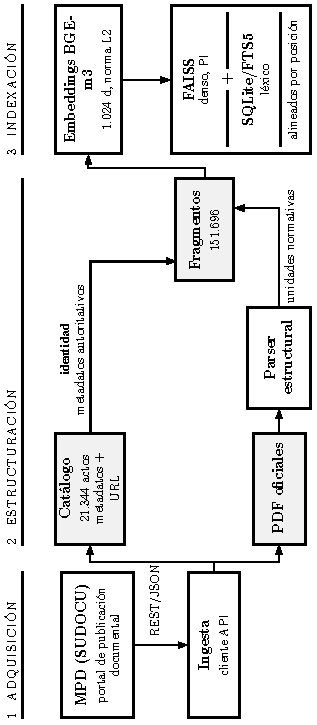
\includegraphics[angle=-90, width=\textwidth]{figs/pipeline-design.pdf}
\caption{Arquitectura de construcci\'on del corpus.}
\label{fig:pipeline}
\end{figure}

% \begin{figure}[H]
% \centering
% \resizebox{\textwidth}{!}{%
% \begin{tikzpicture}[
%   caja/.style={draw, rounded corners=2pt, align=center, font=\scriptsize,
%                inner sep=4pt, minimum height=8mm, minimum width=22mm},
%   dato/.style={font=\tiny\itshape},
%   flecha/.style={-{Stealth[length=2mm]}, semithick}]
% \node[caja] (mpd) at (0,0) {MPD\\ (SUDOCU)};
% \node[caja] (ing) at (3.3,0) {Ingesta\\ (cliente API)};
% \node[caja] (cat) at (7.1,0) {Cat\'alogo: 21.344 actos\\ metadatos + URL};
% \node[caja] (pdf) at (0,-1.9) {PDF oficiales};
% \node[caja] (par) at (3.3,-1.9) {Parser estructural};
% \node[caja] (chk) at (7.1,-1.9) {Fragmentos:\\ 151.696};
% \node[caja] (emb) at (7.1,-3.8) {Embeddings BGE-m3\\ 1.024 d, norma L2};
% \node[caja] (idx) at (10.9,-3.8) {FAISS (denso, PI)\\ SQLite/FTS5 (l\'exico)\\ alineados por posici\'on};
% \draw[flecha] (mpd) -- node[dato, above]{REST/JSON} (ing);
% \draw[flecha] (ing) -- (cat);
% \draw[flecha] (ing) -- (pdf);
% \draw[flecha] (pdf) -- (par);
% \draw[flecha] (par) -- node[dato, above]{unidades} (chk);
% \draw[flecha] (cat) -- node[dato, right]{identidad} (chk);
% \draw[flecha] (chk) -- (emb);
% \draw[flecha] (emb) -- (idx);
% \end{tikzpicture}}
% \caption{Arquitectura de construcci\'on del corpus.}
% \label{fig:pipeline}
% \end{figure}

El parser convierte cada PDF a texto estructurado y lo segmenta por unidad
normativa ---Visto, Considerando, parte resolutiva, art\'iculos, anexos---: la
unidad de recuperaci\'on coincide con la unidad citable, de modo que una
respuesta puede referir el art\'iculo 2 de una disposici\'on y enlazar
exactamente ese texto. Cada fragmento porta la identidad y la trazabilidad del acto ---c\'odigo,
n\'umero, a\~no, fecha, identificadores del portal y URL permanente---, tomadas
del cat\'alogo y no del PDF.



\subsection{Vectorizaci\'on e indexaci\'on}
\label{sec:vectorizacion}

Los \emph{embeddings} se calculan con BGE-m3~\cite{chen2024bge}, modelo
multiling\"ue de recuperaci\'on entrenado contrastivamente sobre pares masivos,
con soporte de representaci\'on densa, dispersa y multivector; se emplea la
representaci\'on densa, de 1.024 dimensiones y normalizada L2, de modo que el
producto interno equivale a la similitud coseno y el \'indice puede ser exacto y
plano. Se vectorizan los 151.696 fragmentos del corpus (7,1 por documento;
55.929 art\'iculos). La ventana de 8.192
tokens admite fragmentos largos sin truncamiento. Cada fragmento se codifica con
un encabezado sint\'etico ---t\'itulo del acto y cita citable, antepuestos al
cuerpo---: un condicionamiento de contexto documental sobre la representaci\'on
local que mitiga la p\'erdida de contexto inherente a la fragmentaci\'on,
en l\'inea con la concatenaci\'on de t\'itulo y pasaje de los recuperadores
densos~\cite{karpukhin2020dpr}. Los artefactos de b\'usqueda son un
\'indice FAISS~\cite{douze2024faiss} de producto interno y una base SQLite con el
texto, los metadatos y un \'indice l\'exico FTS5\footnote{\url{https://sqlite.org/fts5.html}, consultado en agosto de 2026.},
alineados por posici\'on y verificados tras cada reconstrucci\'on; el reemplazo es at\'omico y la API recarga el \'indice sin
interrumpir el servicio. La operaci\'on completa ---cat\'alogo, descarga,
vectorizaci\'on, indexaci\'on--- se ejecuta desde el panel de administraci\'on del
propio sistema, con registro de corridas, y la actualizaci\'on peri\'odica
reutiliza el mismo camino de forma incremental.

% ============================ 4. SISTEMA ============================
\subsection{Recuperaci\'on h\'ibrida}
\label{sec:sistema}

La recuperaci\'on combina la b\'usqueda por \emph{embeddings} de la
Secci\'on~\ref{sec:vectorizacion} con recuperaci\'on l\'exica: una
implementaci\'on propia de BM25~\cite{robertson2009bm25}
($k_1{=}1{,}5$, $b{=}0{,}75$) cuyo tokenizador \emph{preserva los identificadores
normativos} ---expresiones como \texttt{RESHCS-LUJ: 0000042-24}, \texttt{528/2025}
o \texttt{DISPCD-CB} se mantienen como unidades--- porque son exactamente lo que
los \emph{embeddings} no distinguen. Los dos \emph{rankings} se fusionan por
\emph{reciprocal rank fusion} (RRF)~\cite{cormack2009rrf}, que asigna a cada
documento la suma de los rec\'iprocos de su posici\'on en cada \emph{ranking}:
\begin{equation}
\mathrm{RRF}(d) = \sum_{r \in \{\mathrm{emb},\,\mathrm{BM25}\}} \frac{1}{K + \mathrm{rango}_r(d)},
\qquad K = 60,
\label{eq:rrf}
\end{equation}
donde $\mathrm{rango}_r(d)$ es la posici\'on del documento $d$ en el
\emph{ranking} $r$ y la constante $K$ amortigua la diferencia entre las primeras
posiciones. Fusionar por posiciones, y no por puntajes, evita calibrar
magnitudes de naturaleza distinta ---similitud coseno y puntaje BM25---.
Cuando la consulta nombra un acto concreto, la b\'usqueda se restringe a los
documentos que llevan ese n\'umero. La fusi\'on por s\'i sola no lo garantiza: un
documento con posiciones intermedias en ambos \emph{rankings} supera a uno que
encabeza uno solo. Adem\'as,
el n\'umero solo no alcanza, porque cada tipo de acto lleva numeraci\'on propia y
un mismo n\'umero existe en decenas de c\'odigos distintos.

\subsection{Estado de di\'alogo con procedencia}
\label{sec:estado}

En cada turno, una \'unica pasada de un modelo de lenguaje sobre los \'ultimos
intercambios produce conjuntamente una consulta autocontenida y una salida
estructurada con los referentes detectados. La consulta reescrita repone la
informaci\'on omitida en las repreguntas el\'ipticas, mientras que esos mismos
referentes actualizan los \emph{slots} del estado de di\'alogo y permanecen
disponibles para su inspecci\'on, correcci\'on y ponderaci\'on durante los
turnos siguientes.

El estado mantiene dos \emph{slots}. El primero, \emph{entidad}, registra el
sujeto de la conversaci\'on ---una persona, una carrera, una dependencia, un
\'organo---, con cardinalidad uno y sem\'antica de reemplazo. El segundo,
\emph{actos}, acumula el conjunto de actos administrativos mencionados. El
criterio de admisi\'on fue restrictivo: un \emph{slot} se justifica \'unicamente
si transporta entre turnos informaci\'on que el texto de la consulta actual no
contiene.

Los \emph{slots} se muestran sobre el campo de escritura desde la primera
recuperaci\'on y permanecen visibles durante la conversaci\'on. El estado es
editable: quien consulta puede corregir la entidad, descartar un acto o
reincorporarlo. Lo descartado permanece
visible, atenuado, dado que la inspecci\'on de lo inferido es condici\'on para su
control. Cuando una entidad fijada no aparece en la consulta con la que se
buscar\'a, el sistema declara la discrepancia en la interfaz en lugar de
resolverla de manera impl\'icita.

\label{sec:procedencia}Cada valor del estado registra, adem\'as, su
\emph{procedencia}, de la que se deriva su peso en la recuperaci\'on: un valor
inferido por el modelo a partir de la conversaci\'on pesa 0,5; uno fijado
expl\'icitamente por quien consulta pesa 1,0 y deja de ser sobrescrito por la
inferencia en los turnos siguientes; uno descartado pesa 0. El peso entra como
bonificaci\'on aditiva sobre el puntaje fusionado:

\begin{equation}
\mathrm{puntaje}(d) = \mathrm{RRF}(d) + \sum_{s \in S} w_s \cdot \mathbb{1}[\,d \models s\,] \cdot u
\label{eq:puntaje}
\end{equation}

donde $S$ es el conjunto de \emph{slots} activos, $w_s$ el peso derivado de la
procedencia y $u = 1/(K+1)$ la unidad de bonificaci\'on, equivalente a encabezar
uno de los dos \emph{rankings}. Expresarla en unidades de RRF evita una
constante arbitraria y acota el efecto: un \emph{slot} desplaza el ordenamiento,
pero no sustituye a la relevancia, que aporta por ambos \emph{rankings}. La
correcci\'on del usuario opera as\'i como una observaci\'on de mayor confianza
que la inferencia del propio sistema: duplica el peso del valor en la
Ecuaci\'on~\ref{eq:puntaje} y fija su persistencia.

Ning\'un \emph{slot} excluye documentos: un valor mal inferido degrada el
ordenamiento pero no puede anular el conjunto de resultados, el modo de falla
caracter\'istico de los filtros estrictos.

El estado cumple as\'i tres funciones: conserva los referentes que resuelven la
elipsis, expone la interpretaci\'on que el sistema mantiene y admite su
correcci\'on directa; la procedencia de cada valor determina su peso y su
persistencia en la recuperaci\'on.

% ========================== 5. EVALUACION ==========================
\subsection{Generaci\'on}

La respuesta se redacta con un modelo de lenguaje que recibe la consulta, el
contexto recuperado ---fragmentos con su cita--- y la instrucci\'on de respaldar
cada afirmaci\'on con el identificador del acto correspondiente, sin afirmar
nada que el contexto no contenga. El componente es intercambiable: el sistema
admite cualquier \emph{endpoint} compatible con la API de OpenAI ---servicios en
la nube o modelos de pesos abiertos servidos localmente (vLLM, Ollama)--- y se
configura desde el panel de administraci\'on, sin reiniciar el servicio. Sobre
la misma recuperaci\'on, el sistema expone modos de salida invocables por
comandos (\texttt{/lista}, \texttt{/ficha}, \texttt{/comparar},
\texttt{/novedades}, \texttt{/resumen}) que reconfiguran la selecci\'on de
contexto y la instrucci\'on de generaci\'on: inventarios por tema, dossier de un
acto ---incluida la relaci\'on inversa de qu\'e actos lo mencionan, que el portal
no ofrece---, comparaci\'on entre dos actos, novedades por ventana temporal y
s\'intesis narrada.

\subsection{Protocolo de evaluaci\'on}
\label{sec:evaluacion}

Ante la ausencia de un conjunto anotado sobre este corpus, la
recuperaci\'on se eval\'ua con consultas sint\'eticas construidas por muestreo
estratificado por secci\'on del portal y tipo de acto, de tres clases: por
\emph{identificador} ($n=30$; plantillas deterministas sobre el c\'odigo del
acto), por \emph{contenido} ($n=131$; generadas con un modelo de lenguaje a
partir de un fragmento, sin nombrar el n\'umero del acto, con un control de
calidad autom\'atico ---un segundo pase que juzga si el fragmento responde la
consulta--- que descart\'o el 34{,}5\%) y \emph{conversacionales} de dos
turnos ($n=58$; el segundo turno es una repregunta el\'iptica). La relevancia se
decide a nivel de acto ---el sistema cita y enlaza actos completos--- y se
reportan Recall@$k$, MRR@10~\cite{voorhees1999trec} y
nDCG@10~\cite{jarvelin2002cumulated}. La fidelidad de las citas se verifica de
forma determinista: todo acto citado en una respuesta debe estar entre lo
recuperado, y la atribuci\'on a una persona nombrada debe estar contenida en el
fragmento citado\footnote{Tanto la generaci\'on de consultas sint\'eticas como la de
respuestas us\'o \texttt{gpt-4o-mini} a temperatura 0.}.

\label{sec:humana}El juicio humano complementa las m\'etricas autom\'aticas:
tres evaluadores de perfiles distintos ---estudiante, docencia y gesti\'on---
completan un cuestionario \'unico con quince respuestas fijas del sistema
---id\'enticas entre jueces, lo que permite reportar acuerdo--- y tres consultas
propias realizadas en vivo, puntuadas de 1 a 5 en utilidad, fidelidad,
completitud y claridad\footnote{El cuestionario y los \'items evaluados
est\'an disponibles en el repositorio del sistema:
\url{https://github.com/jumafernandez/rag-unlu} (directorio
\texttt{evaluacion/}).}.

% ========================= 6. RESULTADOS =========================
\section{Experimentos y resultados}
\label{sec:resultados}

La evaluaci\'on autom\'atica se centra en la recuperaci\'on: la
Tabla~\ref{tab:ablacion} compara los componentes aislados, la fusi\'on h\'ibrida
y el sistema completo sobre los tres tipos de consulta del protocolo.

\begin{table}[H]
\centering\scriptsize
\caption{Recuperaci\'on por tipo de consulta. En las conversacionales, todas
las configuraciones salvo el sistema completo operan sobre el segundo turno
crudo.}
\label{tab:ablacion}
\begin{tabular*}{\textwidth}{@{\extracolsep{\fill}}lrrrrrrrrr@{}}
\toprule
 & \multicolumn{3}{c}{Identificador} & \multicolumn{3}{c}{Contenido} & \multicolumn{3}{c}{Conversacional} \\
\cmidrule(lr){2-4}\cmidrule(lr){5-7}\cmidrule(l){8-10}
Configuraci\'on & R@5 & MRR & nDCG & R@5 & MRR & nDCG & R@5 & MRR & nDCG \\
\midrule
Solo \emph{embeddings} & 0.10 & 0.08 & 0.08 & 0.78 & 0.65 & 0.69 & 0.10 & 0.08 & 0.09 \\
Solo BM25              & 0.83 & 0.68 & 0.76 & 0.79 & 0.68 & 0.72 & 0.09 & 0.08 & 0.08 \\
H\'ibrido              & 1.00 & 1.00 & 1.00 & 0.82 & 0.72 & 0.75 & 0.12 & 0.08 & 0.09 \\
H\'ibrido $+$ estado & \textbf{1.00} & \textbf{1.00} & \textbf{1.00} & \textbf{0.82} & \textbf{0.72} & \textbf{0.75} & \textbf{0.93} & \textbf{0.88} & \textbf{0.90} \\
\bottomrule
\end{tabular*}
\end{table}

Ninguno de los dos componentes alcanza por s\'i solo: los \emph{embeddings} no
distinguen identificadores normativos y BM25, aun preserv\'andolos, no ordena la
sem\'antica de las consultas por contenido tan bien como la fusi\'on; el
h\'ibrido resuelve por completo las consultas por identificador y conserva la
ventaja en las de contenido. El resultado perfecto de la primera columna se
explica por el anclaje de identificadores que integran las configuraciones
h\'ibridas: cuando la consulta nombra un acto, la b\'usqueda se restringe a los
documentos que llevan ese identificador, y el acto correcto encabeza el
\emph{ranking} con independencia de la fusi\'on; sin esa restricci\'on, la
fusi\'on por posiciones no lo garantiza. En las consultas conversacionales
ancladas en un acto, esa misma restricci\'on se habilita porque el estado repone
el identificador omitido en la consulta reescrita: la composici\'on de ambos
mecanismos explica el 1{,}00 de esa poblaci\'on. La columna conversacional muestra el papel del
estado: sobre el segundo turno crudo ninguna configuraci\'on recupera (R@5 de
0{,}09 a 0{,}12) y el sistema completo alcanza 0{,}93, con la reescritura
condicionada al historial como mecanismo determinante; los \emph{slots}, cuyos
valores ya est\'an repuestos en la consulta reescrita, conservan su funci\'on de
correcci\'on con prioridad garantizada por la procedencia. En la evaluaci\'on
de procedencia, la condici\'on de \emph{estado corregido} ---la entidad fijada
con el peso de una correcci\'on humana--- sostiene los valores de la
configuraci\'on completa (R@5 de 0{,}93; 0{,}86 y 1{,}00 por poblaci\'on), y la
remoci\'on individual de cada \emph{slot} no los altera: m\'as all\'a de las
m\'etricas de recuperaci\'on, la ventaja de la procedencia es habilitar la
correcci\'on humana con prioridad y persistencia garantizadas, una propiedad
del r\'egimen de interacci\'on que el ordenamiento no captura. Un \emph{cross-encoder}
(BGE-reranker-v2-m3) reordenando el top-50 del h\'ibrido no mejora las
m\'etricas (R@1 global de 0{,}68 contra 0{,}70) y empeora los identificadores:
el ordenamiento no es el cuello de botella de este dominio. La
verificaci\'on determinista de citas sobre 60 respuestas ancla el 97{,}0\% de
los actos citados en lo recuperado, con atribuci\'on de personas correcta en 23
de 24 casos.

La validaci\'on humana complementa esas m\'etricas. Los quince \'items fijos
cubren los tres tipos de consulta del protocolo sobre secciones diversas del
corpus, con respuestas verificables en uno o dos actos; cada juez agrega tres
consultas propias de su actividad, realizadas en vivo. La
Tabla~\ref{tab:jueces} resume los puntajes.

\begin{table}[H]
\centering\small
\caption{Validaci\'on con evaluadores: media $\pm$ desv\'io est\'andar por
dimensi\'on sobre los \'items fijos (tres jueces). Los segmentos indican
$\pm$1 DE.}
\label{tab:jueces}
\begin{minipage}[c]{0.40\textwidth}
\centering
\begin{tabular}{lc}
\toprule
Dimensi\'on & Media $\pm$ DE \\
\midrule
Utilidad     & 4,47 $\pm$ 1,11 \\
Fidelidad    & 4,73 $\pm$ 0,58 \\
Completitud  & 4,53 $\pm$ 0,78 \\
Claridad     & 4,77 $\pm$ 0,50 \\
\bottomrule
\end{tabular}
\end{minipage}\hfill
\begin{minipage}[c]{0.56\textwidth}
\centering
\begin{tikzpicture}
\begin{axis}[
  width=\linewidth, height=4.3cm,
  ybar, bar width=10pt,
  ymin=1, ymax=5.7,
  ytick={1,2,3,4,5},
  ymajorgrids, grid style={dashed,black!15},
  axis x line*=bottom, axis y line*=left,
  symbolic x coords={Utilidad,Fidelidad,Completitud,Claridad},
  xtick={Utilidad,Fidelidad,Completitud,Claridad},
  enlarge x limits=0.15,
  x tick label style={rotate=22,anchor=east,font=\scriptsize},
  y tick label style={font=\scriptsize},
]
\addplot[ybar,bar shift=0pt,bar width=16pt,draw=black,fill=black!25,
  error bars/.cd,y dir=both,y explicit,error mark=|,
  error bar style={black},error mark options={black,mark size=3.5pt,line width=0.7pt}] coordinates {
  (Utilidad,4.47) +- (0,1.11)
  (Fidelidad,4.73) +- (0,0.58)
  (Completitud,4.53) +- (0,0.78)
  (Claridad,4.77) +- (0,0.50)
};
\end{axis}
\end{tikzpicture}
\end{minipage}
\end{table}

Las cuatro dimensiones superan 4,4 sobre 5. Fidelidad (4,73 $\pm$ 0,58) y
claridad (4,77 $\pm$ 0,50) concentran los puntajes m\'as altos y los menores
desv\'ios, en l\'inea con la verificaci\'on determinista de citas: las
observaciones de los jueces refieren principalmente omisiones de detalle ---un
identificador no citado, el \'organo firmante ausente--- antes que afirmaciones
contrarias a las fuentes. La mayor dispersi\'on corresponde a utilidad ($\pm$
1,11) y se concentra en los \'items en los que el corpus no contiene normativa
espec\'ifica para la consulta y el sistema respondi\'o con material adyacente en
lugar de declarar la ausencia; los jueces coincidieron en penalizar ese
comportamiento, que constituye la principal l\'inea de mejora observada.

\label{sec:portabilidad}Si bien la evaluaci\'on se realiz\'o sobre la
instalaci\'on de la UNLu ---donde se cuenta con mayor conocimiento del corpus y
acceso a los evaluadores---, la portabilidad t\'ecnica del pipeline se
verific\'o contra el portal SUDOCU de la Universidad Nacional de San Luis. Se gener\'o una
personalizaci\'on con los datos de esa universidad ---identidad institucional,
esquema de colores y URL de su portal--- que permiti\'o construir una instancia
completa desde el propio panel de administraci\'on: el proceso de ingesta
comprob\'o la compatibilidad de la instalaci\'on con tres solicitudes de solo
lectura, descubri\'o autom\'aticamente sus 15 carpetas p\'ublicas ---72.816
actos declarados--- y descarg\'o de forma escalonada, para no saturar el
servidor de origen, los 26.282 documentos de tres carpetas, incluido el
Rectorado, la mayor del portal.

% ======================== 7. CONCLUSIONES ========================
\section{Conclusiones y trabajo futuro}
\label{sec:conclusiones}

Se present\'o un sistema real de consulta conversacional de normativa
universitaria, en operaci\'on sobre el corpus completo de la UNLu y con una
segunda instancia sobre el portal de la UNSL. Los aportes: un estado de
di\'alogo cuya \emph{procedencia} determina el peso de cada valor en la
recuperaci\'on ---visible, editable y con su efecto medido por ablaci\'on---;
una recuperaci\'on h\'ibrida con anclaje de identificadores normativos que
resuelve por completo la consulta por identificador y encabeza la tem\'atica;
una arquitectura de ingesta, indexaci\'on y operaci\'on \'integramente
autoadministrada, portable entre instalaciones de SUDOCU a costo de
configuraci\'on ---un dise\~no pensado para el sistema universitario
argentino---; y correspondencia verificada entre las citas y el material recuperado, con
enlace de cada cita al documento oficial publicado.

Entre las limitaciones: la evaluaci\'on se apoya en consultas sint\'eticas sin
revisi\'on manual, con relevancia referida al acto de origen de cada consulta,
y la evidencia sobre la UNSL se limita a la portabilidad t\'ecnica del
pipeline.

Como trabajo futuro se propone, por un lado, la incorporaci\'on del sistema al
sistema universitario argentino ---despliegue en nuevas instalaciones de SUDOCU
y evaluaci\'on con jueces de cada instituci\'on--- y, por el otro, completar el
corpus de la UNLu con el digesto heredado del sistema anterior, de
aproximadamente 120.000 documentos y otra fisonom\'ia. A ello se suma la explotaci\'on de los
v\'inculos textuales entre actos que el sistema ya extrae ---las menciones
expl\'icitas de modificaci\'on, derogaci\'on o referencia que un acto hace de
otro--- hacia una representaci\'on estructurada del corpus normativo, que
habilitar\'ia consultas hoy fuera de alcance: la cronolog\'ia normativa de un
tema, la trayectoria de una norma a trav\'es de sus modificaciones y la
navegaci\'on por relaciones entre actos.


\subsubsection*{Agradecimientos.}
Esta investigaci\'on se desarroll\'o en el marco de un proyecto apoyado por la
iniciativa IPAC (C\'omputo de Alto Desempe\~no Argentina), convocatoria PCI-146
(Proyectos de C\'omputo Intensivo). Los autores agradecen asimismo al Sistema
Nacional de C\'omputo de Alto Desempe\~no (SNCAD), a la infraestructura
Clementina XXI, a la SICyT y a su equipo t\'ecnico por el apoyo en la
ejecuci\'on de los experimentos, y al CIDETIC (UNLu) por los recursos de
infraestructura provistos para el despliegue institucional del sistema.

\bibliographystyle{splncs03}
\bibliography{References}

\end{document}
